% Drawing 156-1/02-1 -- folder 156-1, batch 02, archive page 25 (PDF page 26).
% Transcription: figure barrée de traits obliques
% Kind: circle x, y with arcs I, J, struck by oblique strokes. Method 2 (schematic redraw from the facsimile). Status: ok.
% Notes: A circle through x (left) and y (right), the upper arc I with an arrowhead towards y, the lower arc J with an arrowhead towards x; the whole struck by four oblique strokes (drawn grey).
% Coordinates: 1 unit = 1 mm = 1/100 of the crop width (bbox in page fractions: [0.42, 0.08, 0.72, 0.24]).
% Redrawn by Claude (claude-opus-5-5), issue #73, 2026-11-07; not checked by a human; not compiled (no TeX in the session).
% Rights: reproduces part of the work -- behind RENDER_TRANSCRIPTS, never published by itself.
\documentclass[tikz,border=3pt]{standalone}
\usepackage{amsmath,amssymb}
\usetikzlibrary{patterns,arrows.meta}
\tikzset{pencil/.style={black!45}, struck/.style={black!35}, mark/.style={circle,draw,inner sep=1.3pt}, pt/.style={circle,fill,inner sep=0.9pt}, opt/.style={circle,draw,fill=white,inner sep=1.1pt}}
\begin{document}
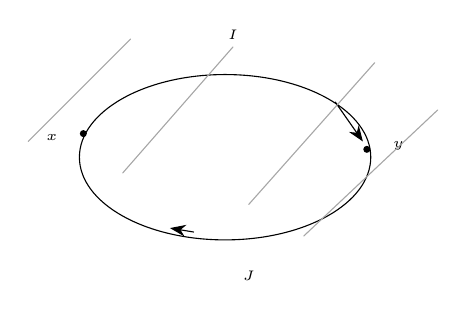
\begin{tikzpicture}[x=1mm,y=1mm,line cap=round,line join=round,font=\scriptsize]
\draw (60,-48) ellipse[x radius=18.5, y radius=10.5];
\node[pt] at (42,-45) {};
\node[pt] at (78,-47) {};
\node[inner sep=1pt] at (38,-45.5) {\tiny $x$};
\node[inner sep=1pt] at (82,-46.5) {\tiny $y$};
\draw[-{Stealth[length=2mm]}] (74,-41) -- (77.5,-46);
\draw[-{Stealth[length=2mm]}] (56,-57.5) -- (53,-57);
\node[inner sep=1pt] at (61,-32.5) {\tiny $I$};
\node[inner sep=1pt] at (63,-63) {\tiny $J$};
\draw[struck] (35,-46) -- (48,-33);
\draw[struck] (47,-50) -- (61,-34);
\draw[struck] (63,-54) -- (79,-36);
\draw[struck] (70,-58) -- (87,-42);
\end{tikzpicture}
\end{document}
